%%%%%%%%%%%%%%%%%%%%%%% file template.tex %%%%%%%%%%%%%%%%%%%%%%%%%
%
% This is a general template file for the LaTeX package SVJour3
% for Springer journals.          Springer Heidelberg 2010/09/16
%
% Copy it to a new file with a new name and use it as the basis
% for your article. Delete % signs as needed.
%
% This template includes a few options for different layouts and
% content for various journals. Please consult a previous issue of
% your journal as needed.
%
% !!! install inkscape and add it to system path and add -shell-escape option to the pdflatex compile command
%
%%%%%%%%%%%%%%%%%%%%%%%%%%%%%%%%%%%%%%%%%%%%%%%%%%%%%%%%%%%%%%%%%%%
%
% First comes an example EPS file -- just ignore it and
% proceed on the \documentclass line
% your LaTeX will extract the file if required
\begin{filecontents*}{example.eps}
%!PS-Adobe-3.0 EPSF-3.0
%%BoundingBox: 19 19 221 221
%%CreationDate: Mon Sep 29 1997
%%Creator: programmed by hand (JK)
%%EndComments
gsave
newpath
  20 20 moveto
  20 220 lineto
  220 220 lineto
  220 20 lineto
closepath
2 setlinewidth
gsave
  .4 setgray fill
grestore
stroke
grestore
\end{filecontents*}
%
\RequirePackage{fix-cm}
%
% \documentclass{report}
%\documentclass{svjour3}                     % onecolumn (standard format)
%\documentclass[smallcondensed]{svjour3}     % onecolumn (ditto)
%\documentclass[smallextended,twocolumn,final]{svjour3}       % onecolumn (second format)
\documentclass[twocolumn]{svjour3}          % twocolumn
%
%\smartqed  % flush right qed marks, e.g. at end of proof


%
\usepackage{mathptmx}      % use Times fonts if available on your TeX system
%
% insert here the call for the packages your document requires
%\usepackage{latexsym}
% etc.


%It is, however, highly recommended to use the fonts with the extended T1 and TS1 (text symbols) encodings by means of the commands:
\usepackage[T1]{fontenc}
\usepackage[utf8]{inputenc}		% Umlaute etc. können direkt eingegeben werden --> changed from utf8x to utf8 because error with biblatex occured
\usepackage{textcomp}
%When using PostScript fonts that come from ‘outside the TEX world’, there is no reason at all to stay with the obsolete OT1 encoding, which would not provide access to all available glyphs. However, since these fonts were not particularly designed for use with TEX, they do not include all of the text companion (TS1) symbols.

%%%% Graphics
\usepackage{lineno}
\linenumbers
\modulolinenumbers[2]

\usepackage{graphicx}
\usepackage{tikz}

\usepackage{enumitem}
\usepackage{bookmark}

\usepackage{grffile}
\usepackage{mathtools}
\usepackage{amssymb}
\usepackage{amsmath}
\usepackage{verbatim}
\usepackage{relsize}
\usepackage[version=4]{mhchem} % for chemical reaction typing

\usepackage{xfrac}
\usepackage[per-mode = fraction,detect-all = true]{siunitx} % per-mode=fraction
\usepackage{xspace} % vereinfachtes Eingeben von Leerschlägen hinter Shortcut-Commands Beispiel: \newcommand{\DNA}{Deso....\xspace}
\usepackage{cancel} % to allow siuntitx to cancel out in equations of units


% !!! install inkscape and add it to system path and add -shell-escape option to the pdflatex compile command
\usepackage{svg}
\usepackage[twoside,figuresright]{rotating} % allows sidewaysfigure environment
\usepackage{afterpage} % To place figure on odd page or even page

\usepackage[colorinlistoftodos,draft]{todonotes}
\reversemarginpar												% bring todonotes to the oposite margin
\setlength{\marginparwidth}{3cm}				% change width of todonotes at the margins

%%%%%%% FOR nice tables %%%%%%%%%%%%
\usepackage{tabularx}
\usepackage{longtable}
\usepackage{booktabs}
\usepackage{multirow}
%%%%%%%%%%%%%%%%%%%%%%%%%%%%%%%%%%%%




%
% please place your own definitions here and don't use \def but
% \newcommand{}{}

%%%%%%%%%%%%%%%%%%%%%%%%%%%%%%%%%%%%%%%%%%%%%%%%%%%%%%%%%%%%%%%%%%%%%%%%%%%%%%%%%%%%%%%%%%%%%%%%%%%%%%%%%%%%%%%%%%
% Text short cuts
%%%%%%%%%%%%%%%%%%%%%%%%%%%%%%%%%%%%%%%%%%%%%%%%%%%%%%%%%%%%%%%%%%%%%%%%%%%%%%%%%%%%%%%%%%%%%%%%%%%%%%%%%%%%%%%%%%
\newcommand{\shortcutexample}[1][]{short cut example{\ifx&#1&{ }\else#1\fi}}

\newcommand{\pthc}{PtG}
\newcommand{\ptg}{PtG}
\newcommand{\ptgas}{Power-to-Gas}
\newcommand{\ptsng}{Power-to-SNG}

\newcommand{\rs}[1]{\relsize{#1}}
\newcommand{\ms}[1]{\mathsmaller{#1}}

\newcommand{\citeA}[2][]{{\citeauthor{#2}{ }\cite[#1]{#2}}}

\newcommand{\fig}[1]{Figure \ref{fig:#1}}
\newcommand{\tab}[1]{Table \ref{tab:#1}}
\newcommand{\equ}[1]{Equation \ref{equ:#1}}

%%%%%%%%%%%%%%%%%%%%%%%%%%%%%%%%%%%%%%%%%%%%%%%%%%%%%%%%%%%%%%%%%%%%%%%%%%%%%%%%%%%%%%%%%%%%%%%%%%%%%%%%%%%%%%%%%%
% SI Einheiten
\AtBeginDocument{\DeclareSIUnit{\kWh}{kWh}}
\AtBeginDocument{\DeclareSIUnit{\MWh}{MWh}}
\AtBeginDocument{\DeclareSIUnit{\GWh}{GWh}}
\AtBeginDocument{\DeclareSIUnit{\TWh}{TWh}}
\AtBeginDocument{\DeclareSIUnit{\ncm}{Nm$^3$}}
\AtBeginDocument{\DeclareSIUnit{\annum}{a}}

\newcommand{\kwhperNcm}[3]{\SI{#1}{\kWh\of{#2}\per\ncm\of{\ce{#3}}}} % not working because parameters can not be used in siunitx without error

\newcommand{\cozwei}{\ce{CO2}}
\newcommand{\hzwei}{\ce{H2}}
\newcommand{\chvier}{\ce{CH4}}

\newcommand{\gram}[2][]{\SI{#2}{\gram\of{#1}}}
\newcommand{\gramCOzwei}[1][]{\gram[\rs{-1}\ce{CO2}]{#1}}

\newcommand{\kwof}[2][]{\SI{#1}{\kilo\watt\of{#2}}\xspace}
\newcommand{\mwof}[2][]{\SI{#1}{\mega\watt\of{#2}}\xspace}
\newcommand{\gwof}[2][]{\SI{#1}{\giga\watt\of{#2}}\xspace}

\newcommand{\kwel}[1][]{\kwof[#1]{el}}
\newcommand{\mwel}[1][]{\mwof[#1]{el}}
\newcommand{\gwel}[1][]{\gwof[#1]{el}}

\newcommand{\mwsng}[1][]{\mwof[#1]{\relsize{-1} SNG}}
\newcommand{\gwsng}[1][]{\gwof[#1]{\relsize{-1} SNG}}

\newcommand{\mwHzwei}[1][]{\mwof[#1]{\ce{H2}}}
\newcommand{\gwHzwei}[1][]{\gwof[#1]{\ce{H2}}}

\newcommand{\kwhel}[1][]{\SI{#1}{\kWh\of{el}}\xspace}
\newcommand{\mwhel}[1][]{\SI{#1}{\MWh\of{el}}\xspace}
\newcommand{\gwhel}[1][]{\SI{#1}{\GWh\of{el}}\xspace}
\newcommand{\twhel}[1][]{\SI{#1}{\TWh\of{el}}\xspace}

\newcommand{\kwhhyd}[1][]{\SI{#1}{\kWh\of{\ce{H2}}}\xspace}
\newcommand{\mwhhyd}[1][]{\SI{#1}{\MWh\of{\ce{H2}}}\xspace}
\newcommand{\gwhhyd}[1][]{\SI{#1}{\GWh\of{\ce{H2}}}\xspace}
\newcommand{\twhhyd}[1][]{\SI{#1}{\TWh\of{\ce{H2}}}\xspace}

\newcommand{\kwhsng}[1][]{\SI{#1}{\kWh\of{\relsize{-1} SNG}}\xspace}
\newcommand{\mwhsng}[1][]{\SI{#1}{\MWh\of{\relsize{-1} SNG}}\xspace}
\newcommand{\gwhsng}[1][]{\SI{#1}{\GWh\of{\relsize{-1} SNG}}\xspace}
\newcommand{\twhsng}[1][]{\SI{#1}{\TWh\of{\relsize{-1} SNG}}\xspace}

\newcommand{\kwhth}[1][]{\SI{#1}{\kWh\of{\relsize{-1} th}}\xspace}


\newcommand{\tCOzwei}[1][]{\SI{#1}{\tonne\of{\relsize{-1}\ce{CO2}}}}

\newcommand{\tonsof}[2]{\SI{#1}{\tonne\of{\relsize{-1}\ce{#2}}}}
\newcommand{\kgof}[2][]{\SI{#1}{\kilogram\of{\relsize{-1}#2}}}

\newcommand{\MiotCOzwei}[1]{#1\,Mio.\,\tCOzwei}

\newcommand{\kwhperkilogram}[3]{\SI{#1}{\kWh\of{#2}\per\kilogram\of{\ce{#3}}}}
\newcommand{\normcubicmetrehour}[2]{\SI{#1}{N\cubic\metre\of{\ce{#2}}\per\hour}}

%%%%%%%%%%%%%%%%%%%%%%%%%%%%%%%%%%%%%%%%%%%%%%%%%%%%%%%%%%%%%%%%%%%%%%%%%%%%%%%%%%%%%%%%%%%%%%%%%%%%%%%%%%%%%%%%%%



%%%%%%%%%%%%%%%%%%%%%%%%%%%%%%%%%%%%%%%%%%%%%%%%%%%%%%%%%%%%%%%%%%%%%%%%%%%%%%%%%%%%%%%%%%%%%%%%%%%%%%%%%%%%%%%%%%

% Numbered circles definition for svg pictures

\usetikzlibrary{shapes,snakes}
\newcommand*\circled[1]{\tikz[baseline=(char.base)]{
		\node[shape=circle,scale=0.8,draw,inner sep=2pt] (char) {#1};}}
\newcommand*\diam[1]{\tikz[baseline=(char.base)]{
		\node[shape=diamond,scale=0.75,draw,inner sep=1pt] (char) {#1};}}

%%%%%%%%%%%%%%%%%%%%%%%%%%%%%%%%%%%%%%%%%%%%%%%%%%%%%%%%%%%%%%%%%%%%%%%%%%%%%%%%%%%%%%%%%%%%%%%%%%%%%%%%%%%%%%%%%%
% New table column type definitions
%%%%%%%%%%%%%%%%%%%%%%%%%%%%%%%%%%%%%%%%%%%%%%%%%%%%%%%%%%%%%%%%%%%%%%%%%%%%%%%%%%%%%%%%%%%%%%%%%%%%%%%%%%%%%%%%%%
\newcolumntype{C}[1]{>{\centering\arraybackslash}m{#1}}
\newcolumntype{V}[1]{>{\small\centering\arraybackslash}m{#1}}
\newcolumntype{L}[1]{>{\raggedright\arraybackslash}m{#1}}
\newcolumntype{K}[1]{>{\raggedright\arraybackslash}p{#1}}
\newcolumntype{k}[1]{>{\small\raggedright\arraybackslash}p{#1}}
\newcolumntype{R}[1]{>{\raggedleft\arraybackslash}p{#1}}
\newcolumntype{Y}{>{\centering\arraybackslash}X}

%\renewcommand{\tabularxcolumn}[1]{m{#1}}

%_________________________________________________________________________________________________________________


%%%%%%%%%%%%%%%%%%%%%%%%%%%%%%%%%%%%%%%%%%%%%%%%%%%%%%%%%%%%%%%%%%%%%%%%%%%%%%%%%%%%%%%%%%%%%%%%%%%%%%%%%%%%%%%%%%
% Define commands for siunitx package
%%%%%%%%%%%%%%%%%%%%%%%%%%%%%%%%%%%%%%%%%%%%%%%%%%%%%%%%%%%%%%%%%%%%%%%%%%%%%%%%%%%%%%%%%%%%%%%%%%%%%%%%%%%%%%%%%%

\newcommand{\tempC}[1]{\SI{#1}{\celsius}}

%_________________________________________________________________________________________________________________



%%%%%%%%%%%%%%%%%%%%%%%%%%%%%%%%%%%%%%%%%%%%%%%%%%%%%%%%%%%%%%%%%%%%%%%%%%%%%%%%%%%%%%%%%%%%%%%%%%%%%%%%%%%%%%%%%%
% TODO notes commands
%%%%%%%%%%%%%%%%%%%%%%%%%%%%%%%%%%%%%%%%%%%%%%%%%%%%%%%%%%%%%%%%%%%%%%%%%%%%%%%%%%%%%%%%%%%%%%%%%%%%%%%%%%%%%%%%%%
%%%%%%%%%%%%%%
% Colors
\definecolor{mygreen}{RGB}{0,105,0}
\definecolor{myred}{RGB}{250,0,0}
\definecolor{nitrogengreen}{RGB}{0,130,60}
\definecolor{methaneorange}{RGB}{246,135,18}
\definecolor{hydrogenred}{RGB}{237,28,36}
\definecolor{cdioxblue}{RGB}{46,49,146}
\definecolor{cmonoxblue}{RGB}{0,173,239}
%%%%%%%%%%%%%%

\newcommand{\onlydraft}[1]{\ifoptionfinal{}{#1}}
\newcommand{\GUIDE}[2][]{{\todo[inline,color=cyan,#1]{\textit{\textcolor{black}{\underline{STORY LINE:}\\ #2}}}}}

\newcommand{\KEYMESSAGE}[2][]{{\todo[inline,color=orange,#1]{\textit{\textcolor{black}{\underline{KEY MESSAGE:}\\ #2}}}}}
\newcommand{\KEYWORD}[1]{\todo[inline,color=cyan]{\textit{\textcolor{black}{\underline{KEY WORD(s):}\\ #1}}}}
\newcommand{\INFO}[2][]{\todo[inline,color=yellow,#1]{\textit{\textcolor{black}{\underline{INFO:}\\ #1}}}}
\newcommand{\TODO}[2][]{{\todo[inline,color=myred,#1]{{\it\color{black}\underline{TO DO:}\newline #2}}}}

\newcommand{\ASK}[3][]{\todo[inline,color=magenta,#1]{\textit{\textcolor{black}{\underline{ASK #2:}\\ #3}}}}

\newcommand{\notiz}[2][]{{\todo[size=\small,#1]{#2}}}
\newcommand{\notizinline}[1]{\notiz[inline]{{\textbullet} #1}}

\newcommand{\mref}[1]{[missing ref: #1 \ref{#1}]}

\newcommand{\platzhalter}[1]{\textit{\textcolor{blue}{\underline{PLATZHALTER:} #1}}}

\newcommand{\bp}[1]{\textbullet #1\\}
\newcommand{\bpdone}[1]{\checkmark \pbox[t]{.9\columnwidth}{\scriptsize \sout{#1}}\\}

\newcommand{\BP}[2][]{\GUIDE[#1]{\bp{#2}}}
\newcommand{\BPdone}[2][]{\GUIDE[#1]{\bpdone{#2}}}

%_________________________________________________________________________________________________________________

%
% Insert the name of "your journal" with
% \journalname{myjournal}
%

\begin{document}

\title{$title$ Data-driven spatio-temporal assessment of surplus electricity potentials in Switzerland for potential use in Power-to-Gas systems
	\thanks{Grants or other notes
about the article that should go on the front page should be
placed here. General acknowledgments should be placed at the end of the article.}
}
%\subtitle{Considering the phase-out of nuclear power, increasing installed photovoltaic capacities and the influence of weather on the energy production.}

%\titlerunning{Short form of title}        % if too long for running head

\author{Sinan L. Teske         \and
        Martin Rüdisüli  %etc.
}


%\authorrunning{Short form of author list} % if too long for running head
% 
% \institute{F. Author \at
%               first address \\
%               Tel.: +123-45-678910\\
%               Fax: +123-45-678910\\
%               \email{fauthor@example.com}           %  \\
% %             \emph{Present address:} of F. Author  %  if needed
%            \and
%            S. Author \at
%               second address
% }

\date{Received: date / Accepted: date}
% The correct dates will be entered by the editor


\maketitle




\begin{abstract}
$abstract$

Insert your abstract here. Include keywords, PACS and mathematical
subject classification numbers as needed.
% \keywords{First keyword \and Second keyword \and More}
% \PACS{PACS code1 \and PACS code2 \and more}
% \subclass{MSC code1 \and MSC code2 \and more}
\end{abstract}

% \clearpage
% \todototoc
% \listoftodos
% \clearpage

$body$


%%%%%%%%%% Examples %%%%%%%%%%%%%%%%%%%%%%%%%%%%%%%%%%%%%%%%%%%%%%%%%%%%%%%%%%%%%%

%\section{Section title}
%\label{sec:1}
%Text with citations \cite{RefB} and \cite{RefJ}.
%\subsection{Subsection title}
%\label{sec:2}
%as required. Don't forget to give each section
%and subsection a unique label (see Sect.~\ref{sec:1}).
%\paragraph{Paragraph headings} Use paragraph headings as needed.
%\begin{equation}
%a^2+b^2=c^2
%\end{equation}
%
%% For one-column wide figures use
%\begin{figure}
%% Use the relevant command to insert your figure file.
%% For example, with the graphicx package use
%  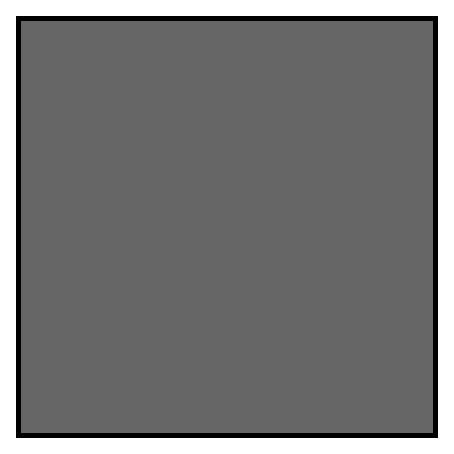
\includegraphics{example.eps}
%% figure caption is below the figure
%\caption{Please write your figure caption here}
%\label{fig:1}       % Give a unique label
%\end{figure}
%%
%% For two-column wide figures use
%\begin{figure*}
%% Use the relevant command to insert your figure file.
%% For example, with the graphicx package use
%  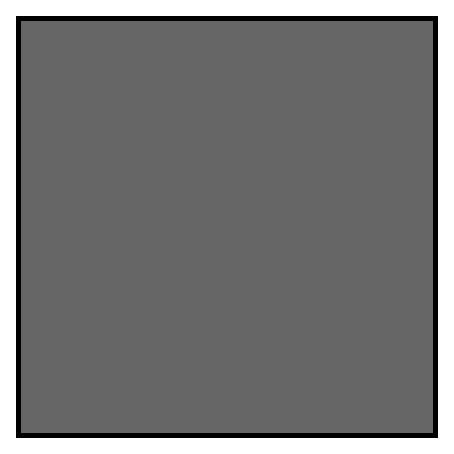
\includegraphics[width=0.75\textwidth]{example.eps}
%% figure caption is below the figure
%\caption{Please write your figure caption here}
%\label{fig:2}       % Give a unique label
%\end{figure*}
%%
%% For tables use
%\begin{table}
%% table caption is above the table
%\caption{Please write your table caption here}
%\label{tab:1}       % Give a unique label
%% For LaTeX tables use
%\begin{tabular}{lll}
%\hline\noalign{\smallskip}
%first & second & third  \\
%\noalign{\smallskip}\hline\noalign{\smallskip}
%number & number & number \\
%number & number & number \\
%\noalign{\smallskip}\hline
%\end{tabular}
%\end{table}
%%%%%%%%%%%%%%%%%%%%%%%%%%%%%%%%%%%%%%%%%%%%%%%%%%%%%%%%%%%%%%%%%%%%%%%%%%%%%%%%%%


% \begin{acknowledgements}
% If you'd like to thank anyone, place your comments here
% and remove the percent signs.
% \end{acknowledgements}

% BibTeX users please use one of
\clearpage
\bibliographystyle{spbasic}      % basic style, author-year citations
% \bibliographystyle{spmpsci}      % mathematics and physical sciences
%\bibliographystyle{spphys}       % APS-like style for physics
% \bibliography{AllDocuments}   % name your BibTeX data base

%% Non-BibTeX users please use OR first draft
%\begin{thebibliography}{}
%
% and use \bibitem to create references. Consult the Instructions
% for authors for reference list style.
%

%\bibitem{Swissgrid2014}
%Swissgrid. Energy statistics Switzerland 2014. 2014. https://www.swissgrid. ch/swissgrid/en/home/reliability/griddata/load.html


%%%%%%%%%%%% Examples %%%%%%%%%%%%%%%%%%%%%%
%\bibitem{RefJ}
%% Format for Journal Reference
%Author, Article title, Journal, Volume, page numbers (year)
%% Format for books
%\bibitem{RefB}
%Author, Book title, page numbers. Publisher, place (year)
%% etc
%%%%%%%%%%%%%%%%%%%%%%%%%%%%%%%%%%%%%%%%%%%%

%\end{thebibliography}

\end{document}
% end of file template.tex

